\section{Per-Seed Results}
\label{sec:appendix-per-seed}

Table~\ref{tab:per-seed-appendix} reports the raw per-seed test weighted F1 for every run cited in the main tables, for direct reproducibility of every mean$\pm$std figure quoted in the text.

\begin{table}[t]
\centering
\caption{Per-seed appendix: raw test weighted F1 for every run cited in the main tables.}
\label{tab:per-seed-appendix}
\begin{tabular}{llc}
\toprule
config & seed & test weighted F1 \\
\midrule
MELD text anchor & 42 & 0.6353 \\
 & 1337 & 0.6441 \\
 & 2024 & 0.6415 \\
MELD full\_R (k=8) & 42 & 0.6374 \\
 & 1337 & 0.6273 \\
 & 2024 & 0.6384 \\
MELD minus\_relational\_R & 42 & 0.6380 \\
 & 1337 & 0.6388 \\
 & 2024 & 0.6329 \\
MELD base\_fusion\_R & 42 & 0.6379 \\
 & 1337 & 0.6399 \\
 & 2024 & 0.6398 \\
IEMOCAP text anchor & 42 & 0.5815 \\
 & 1337 & 0.5939 \\
 & 2024 & 0.5618 \\
IEMOCAP full\_R & 42 & 0.5881 \\
 & 1337 & 0.5832 \\
 & 2024 & 0.5881 \\
IEMOCAP minus\_relational\_R & 42 & 0.6383 \\
 & 1337 & 0.6326 \\
 & 2024 & 0.5887 \\
IEMOCAP base\_fusion\_R & 42 & 0.5970 \\
 & 1337 & 0.6492 \\
 & 2024 & 0.6436 \\
\bottomrule
\end{tabular}
\end{table}


\section{Trained Logit Adjustment: Full Negative Result}
\label{sec:appendix-logit-adjustment}

Section~\ref{sec:meld-foundation} reports in brief that training-time logit adjustment~\cite{menon2021logitadjustment} failed on the rarest MELD classes; the full negative result is recorded here. Training-time logit adjustment, subtracting $\tau \log \pi_c$ from the logits inside the loss, failed in our setting in a specific and diagnosable way: under the trained-adjustment variant, the two rarest classes were ranked last among seven classes by the raw logits for $82\%$ and $69\%$ of their test instances respectively, and no inference-time correction could recover them. Plain cross-entropy training with post-hoc logit adjustment at inference (the estimator's alternative form) moved those ranks to the top three-to-four and left both classes with nonzero F1 in every seed. We report this negative result because trained logit adjustment is widely cited and its silent failure mode, excellent aggregate metrics with structurally dead rare classes, is easy to miss.

\section{Non-Zero Residual Initialization Control}
\label{sec:appendix-nonzero-init}

Section~\ref{sec:residual-construction} notes that the residual construction's exact-zero initialization of $W_{\text{out}}$ and the audio/video fusion blocks is a soft prior toward the foundation, and reports that a small non-zero-init control rules out gradient starvation as an alternative explanation of the fine-tuned-regime null. Table~\ref{tab:nonzero-init-paired-gain} gives the paired gain under both initializations; Table~\ref{tab:nonzero-init-gradients} gives the epoch-0 gradient norms (first 5 training batches, pre-clip) on $W_{\text{out}}$ and the audio/video fusion blocks under both. All 20 captured batches, both conditions, all seeds, have strictly positive $W_{\text{out}}$ and fusion-A/V gradient norms: gradients reach these parameters from the first training batch regardless of initialization scale.

\begin{table*}[t]
\centering
\caption{Non-zero-init control: paired gain (Full stack vs.\ Text-only anchor) on the fine-tuned MELD foundation, exact-zero-init vs.\ a small-scale random ($\mathcal{N}(0, 0.02^2)$) initialization of $W_{\text{out}}$ and the audio/video fusion blocks.}
\label{tab:nonzero-init-paired-gain}
\begin{tabular}{lccc}
\toprule
condition & Full stack mean & paired gain & $n$ \\
\midrule
zero-init (original) & 0.6344 & $-0.0060 \pm 0.0098$ & 3 \\
non-zero-init (control) & 0.6383 & $-0.0020 \pm 0.0044$ & 3 \\
\bottomrule
\end{tabular}
\end{table*}

\begin{table*}[t]
\centering
\caption{Epoch-0 gradient norms (first 5 training batches, pre-clip, mean $\pm$ std) on $W_{\text{out}}$ (the residual classifier) and the audio/video fusion blocks, zero-init vs.\ non-zero-init.}
\label{tab:nonzero-init-gradients}
\begin{tabular}{lcccc}
\toprule
condition & seed & $\lVert\nabla W_{\text{out}}\rVert$ & $\lVert\nabla \text{fusion}_{AV}\rVert$ & $\lVert\nabla \text{total}\rVert$ \\
\midrule
zero-init & 42 & $0.1719 \pm 0.0287$ & $0.0596 \pm 0.0297$ & $0.2627 \pm 0.0438$ \\
non-zero-init & 42 & $0.2156 \pm 0.0344$ & $0.1012 \pm 0.0081$ & $0.3750 \pm 0.0392$ \\
non-zero-init & 1337 & $0.2245 \pm 0.0591$ & $0.1071 \pm 0.0139$ & $0.3950 \pm 0.0689$ \\
non-zero-init & 2024 & $0.1839 \pm 0.0221$ & $0.0999 \pm 0.0125$ & $0.3532 \pm 0.0396$ \\
\bottomrule
\end{tabular}
\end{table*}


\section{Edge-State Trajectories: Qualitative Figure}
\label{sec:appendix-edge-norm}

Section~\ref{sec:iemocap} points here for a qualitative visualization of the relational memory's edge-state norm over dialogue time. Figure~\ref{fig:edge-norm} traces the relational edge-state norm across three complete Session~5 dialogues. The trajectories are structured rather than degenerate: all three dialogues show a rapid rise from an initialization near $0.9$--$1.1$ to a working range of roughly $2.2$--$3.1$, steepest in the first four to five turns and tapering to a slower climb by turn $5$--$7$ in two of the three dialogues and by roughly turn $12$ in the third, then settle into a comparatively stable regime for the remainder of the dialogue: turn-to-turn variance in the second half of each dialogue is $1.8\times$--$7.4\times$ lower than in the first half ($0.454\to0.061$, $0.35\to0.19$, and $0.304\to0.046$ across the three dialogues). The memory is demonstrably accumulating something during an early ``relationship-formation'' phase and then holding it, rather than staying flat at initialization or diverging, which anticipates the dissociation developed in Section~\ref{sec:analysis}: the relational states carry genuine conversational-dynamics information (they \textit{improve} the auxiliary shift-detection task on both corpora) that the emotion readout, resting on a fine-tuned foundation, cannot convert into classification gains. \textbf{One honest caveat, not resolved by the data alone}: a rise-then-plateau shape is also the generic saturation behavior of a GRU-updated state driven by roughly-stationary input statistics, so this pattern is \textit{consistent with} the edge state tracking something relationship-specific but does not on its own \textit{distinguish} that from a purely mechanical settling effect common to recurrent architectures regardless of what they're modeling. We do not believe this figure should be dropped (it directly answers the pre-registered qualitative-artifact commitment and is not degenerate), but whether to present it as evidence of relationship-tracking specifically, versus a more neutral ``the memory is non-trivially stateful'' framing, is an interpretive call the authors resolve at the editing stage rather than settle by construction here. This trajectory is illustrative of the relational memory's operation, not evidence of its value: the quantitative tables in Section~\ref{sec:iemocap} and Section~\ref{sec:analysis} carry that burden, and they carry it in the negative direction.

\begin{figure}[t]
\centering
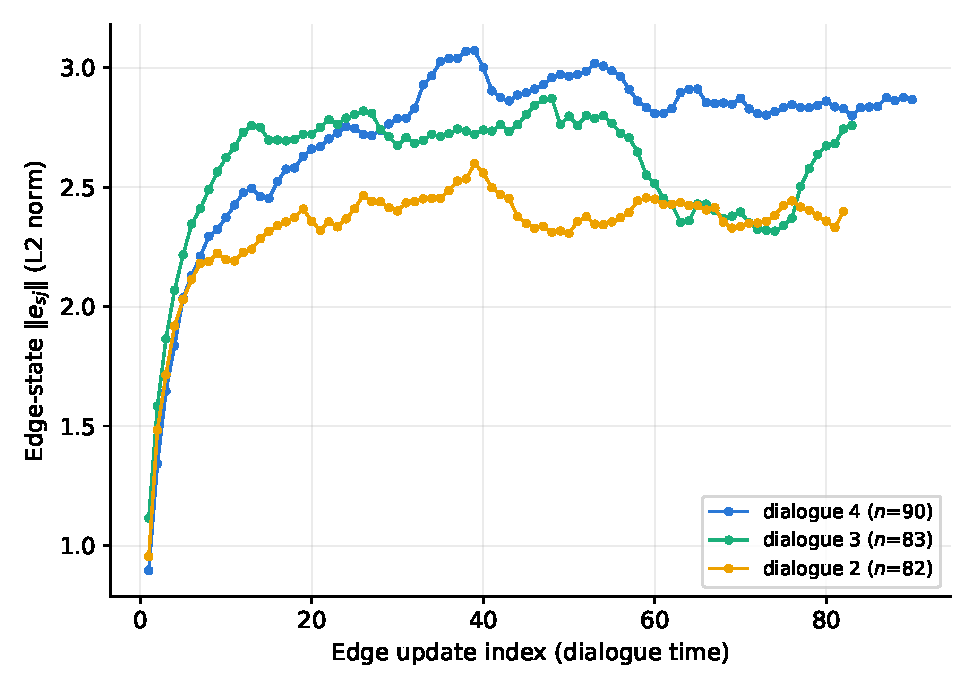
\includegraphics[width=\columnwidth]{figures/edge_state_trajectory.pdf}
\caption{Relational edge-state $L_2$ norm over dialogue time (edge update index, one per speaking turn), three complete Session~5 IEMOCAP dialogues, Full stack configuration, seed $42$. Each trace rises from an initialization near $1.0$ to a working range of roughly $2.2$--$3.1$ and then plateaus with markedly lower turn-to-turn variance in the second half. As discussed in Section~\ref{sec:analysis}, this trajectory is illustrative of the relational memory's operation, not evidence of its value: whether the shape reflects relationship-specific tracking or generic recurrent saturation is not resolved by the plot alone.}
\label{fig:edge-norm}
\end{figure}
